\documentclass[12pt]{extarticle}
\usepackage[T1]{fontenc}
\usepackage{tgheros}
\renewcommand{\familydefault}{\sfdefault}
\usepackage[letterpaper,left=0.75in,right=0.75in,top=0.8in,bottom=0.8in,
  headheight=16pt,headsep=16pt,footskip=28pt]{geometry}
\usepackage{tikz}
\definecolor{slotred}{RGB}{248,182,182}
\definecolor{slotblue}{RGB}{112,152,228}
\usepackage{array}
\usepackage{fancyhdr}
\pagestyle{fancy}
\fancyhf{}
\fancyhead[L]{\normalsize Week NN / Towers from either end / Grades 2--3}
\fancyfoot[L]{\small Bellingham Math Circle / Week NN / NN-23-v1}
\fancyfoot[R]{\small \thepage}
\renewcommand{\headrulewidth}{0pt}
\setlength{\parindent}{0pt}
\setlength{\parskip}{5pt}
\newcounter{prob}
\newcommand{\problem}{\par\bigskip\stepcounter{prob}\noindent\textbf{Problem \theprob:} }
\newcommand{\ruledlines}[2]{\par\noindent\begin{tikzpicture}
  \foreach \k in {1,...,#1}{\draw[black!35] (0,-\k*#2) -- (\linewidth-1pt,-\k*#2);}
  \end{tikzpicture}\par}
\begin{document}

Build the towers on a strip of slots and play with a partner. Take turns. On
your turn, take one whole tower from either end of the row. When the row is
empty, the player with more cubes wins. The same number of cubes is a tie.
Playing as well as you can means collecting as many cubes as you can be sure
of. A row can be written with its heights:
\par\smallskip
\centerline{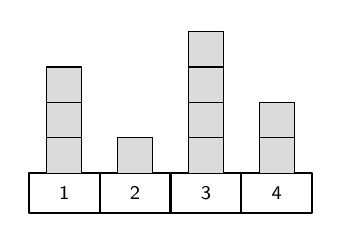
\begin{tikzpicture}[x=1mm,y=1mm,line join=round]
\path (0,0) rectangle (36,23.5);
\draw[thick, fill=white] (0,0) rectangle (9,5);
\node[font=\scriptsize] at (4.5,2.5) {1};
\draw[fill=black!14] (2.25,5.0) rectangle (6.75,9.5);
\draw[fill=black!14] (2.25,9.5) rectangle (6.75,14.0);
\draw[fill=black!14] (2.25,14.0) rectangle (6.75,18.5);
\draw[thick, fill=white] (9,0) rectangle (18,5);
\node[font=\scriptsize] at (13.5,2.5) {2};
\draw[fill=black!14] (11.25,5.0) rectangle (15.75,9.5);
\draw[thick, fill=white] (18,0) rectangle (27,5);
\node[font=\scriptsize] at (22.5,2.5) {3};
\draw[fill=black!14] (20.25,5.0) rectangle (24.75,9.5);
\draw[fill=black!14] (20.25,9.5) rectangle (24.75,14.0);
\draw[fill=black!14] (20.25,14.0) rectangle (24.75,18.5);
\draw[fill=black!14] (20.25,18.5) rectangle (24.75,23.0);
\draw[thick, fill=white] (27,0) rectangle (36,5);
\node[font=\scriptsize] at (31.5,2.5) {4};
\draw[fill=black!14] (29.25,5.0) rectangle (33.75,9.5);
\draw[fill=black!14] (29.25,9.5) rectangle (33.75,14.0);
\end{tikzpicture}\hspace{6mm}\raisebox{6mm}{\tikz[x=1mm,y=1mm]\draw[-latex, black!60, thick] (0,0) -- (9,0);}\hspace{6mm}\raisebox{3mm}{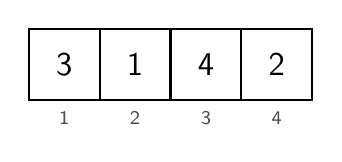
\begin{tikzpicture}[x=1mm,y=1mm]
\draw[thick, fill=white] (0,0) rectangle (9,9);
\node[font=\large] at (4.5,4.5) {3};
\node[font=\scriptsize, black!70] at (4.5,-2.3) {1};
\draw[thick, fill=white] (9,0) rectangle (18,9);
\node[font=\large] at (13.5,4.5) {1};
\node[font=\scriptsize, black!70] at (13.5,-2.3) {2};
\draw[thick, fill=white] (18,0) rectangle (27,9);
\node[font=\large] at (22.5,4.5) {4};
\node[font=\scriptsize, black!70] at (22.5,-2.3) {3};
\draw[thick, fill=white] (27,0) rectangle (36,9);
\node[font=\large] at (31.5,4.5) {2};
\node[font=\scriptsize, black!70] at (31.5,-2.3) {4};
\end{tikzpicture}}}
\problem Play each row twice, so that each of you goes first once. Write both players' totals.\par\vspace{3mm}\noindent\hspace*{18mm}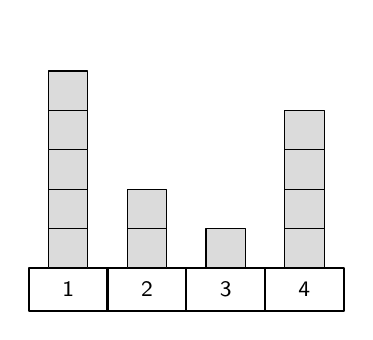
\begin{tikzpicture}[x=1mm,y=1mm,line join=round]
\path (0,0) rectangle (40,36.0);
\draw[thick, fill=white] (0,0) rectangle (10,5.5);
\node[font=\footnotesize] at (5.0,2.75) {1};
\draw[fill=black!14] (2.5,5.5) rectangle (7.5,10.5);
\draw[fill=black!14] (2.5,10.5) rectangle (7.5,15.5);
\draw[fill=black!14] (2.5,15.5) rectangle (7.5,20.5);
\draw[fill=black!14] (2.5,20.5) rectangle (7.5,25.5);
\draw[fill=black!14] (2.5,25.5) rectangle (7.5,30.5);
\draw[thick, fill=white] (10,0) rectangle (20,5.5);
\node[font=\footnotesize] at (15.0,2.75) {2};
\draw[fill=black!14] (12.5,5.5) rectangle (17.5,10.5);
\draw[fill=black!14] (12.5,10.5) rectangle (17.5,15.5);
\draw[thick, fill=white] (20,0) rectangle (30,5.5);
\node[font=\footnotesize] at (25.0,2.75) {3};
\draw[fill=black!14] (22.5,5.5) rectangle (27.5,10.5);
\draw[thick, fill=white] (30,0) rectangle (40,5.5);
\node[font=\footnotesize] at (35.0,2.75) {4};
\draw[fill=black!14] (32.5,5.5) rectangle (37.5,10.5);
\draw[fill=black!14] (32.5,10.5) rectangle (37.5,15.5);
\draw[fill=black!14] (32.5,15.5) rectangle (37.5,20.5);
\draw[fill=black!14] (32.5,20.5) rectangle (37.5,25.5);
\end{tikzpicture}\hspace{24mm}\raisebox{3mm}{{\small\renewcommand{\arraystretch}{1.9}\begin{tabular}{l|p{17mm}|p{17mm}|}\multicolumn{1}{l}{} & \multicolumn{1}{c}{went first} & \multicolumn{1}{c}{went second}\\ \cline{2-3}game 1 & & \\ \cline{2-3}game 2 & & \\ \cline{2-3}\end{tabular}}}\par\vspace{5mm}\noindent\hspace*{18mm}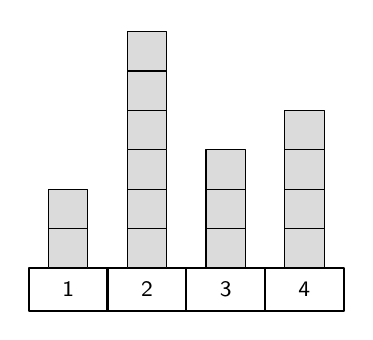
\begin{tikzpicture}[x=1mm,y=1mm,line join=round]
\path (0,0) rectangle (40,36.0);
\draw[thick, fill=white] (0,0) rectangle (10,5.5);
\node[font=\footnotesize] at (5.0,2.75) {1};
\draw[fill=black!14] (2.5,5.5) rectangle (7.5,10.5);
\draw[fill=black!14] (2.5,10.5) rectangle (7.5,15.5);
\draw[thick, fill=white] (10,0) rectangle (20,5.5);
\node[font=\footnotesize] at (15.0,2.75) {2};
\draw[fill=black!14] (12.5,5.5) rectangle (17.5,10.5);
\draw[fill=black!14] (12.5,10.5) rectangle (17.5,15.5);
\draw[fill=black!14] (12.5,15.5) rectangle (17.5,20.5);
\draw[fill=black!14] (12.5,20.5) rectangle (17.5,25.5);
\draw[fill=black!14] (12.5,25.5) rectangle (17.5,30.5);
\draw[fill=black!14] (12.5,30.5) rectangle (17.5,35.5);
\draw[thick, fill=white] (20,0) rectangle (30,5.5);
\node[font=\footnotesize] at (25.0,2.75) {3};
\draw[fill=black!14] (22.5,5.5) rectangle (27.5,10.5);
\draw[fill=black!14] (22.5,10.5) rectangle (27.5,15.5);
\draw[fill=black!14] (22.5,15.5) rectangle (27.5,20.5);
\draw[thick, fill=white] (30,0) rectangle (40,5.5);
\node[font=\footnotesize] at (35.0,2.75) {4};
\draw[fill=black!14] (32.5,5.5) rectangle (37.5,10.5);
\draw[fill=black!14] (32.5,10.5) rectangle (37.5,15.5);
\draw[fill=black!14] (32.5,15.5) rectangle (37.5,20.5);
\draw[fill=black!14] (32.5,20.5) rectangle (37.5,25.5);
\end{tikzpicture}\hspace{24mm}\raisebox{3mm}{{\small\renewcommand{\arraystretch}{1.9}\begin{tabular}{l|p{17mm}|p{17mm}|}\multicolumn{1}{l}{} & \multicolumn{1}{c}{went first} & \multicolumn{1}{c}{went second}\\ \cline{2-3}game 1 & & \\ \cline{2-3}game 2 & & \\ \cline{2-3}\end{tabular}}}\par\vspace{5mm}\noindent\hspace*{18mm}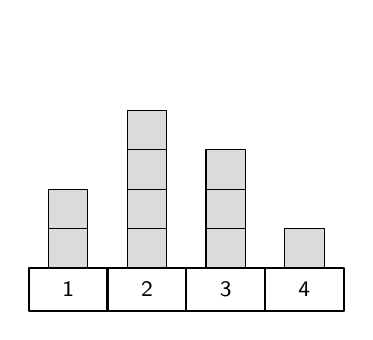
\begin{tikzpicture}[x=1mm,y=1mm,line join=round]
\path (0,0) rectangle (40,36.0);
\draw[thick, fill=white] (0,0) rectangle (10,5.5);
\node[font=\footnotesize] at (5.0,2.75) {1};
\draw[fill=black!14] (2.5,5.5) rectangle (7.5,10.5);
\draw[fill=black!14] (2.5,10.5) rectangle (7.5,15.5);
\draw[thick, fill=white] (10,0) rectangle (20,5.5);
\node[font=\footnotesize] at (15.0,2.75) {2};
\draw[fill=black!14] (12.5,5.5) rectangle (17.5,10.5);
\draw[fill=black!14] (12.5,10.5) rectangle (17.5,15.5);
\draw[fill=black!14] (12.5,15.5) rectangle (17.5,20.5);
\draw[fill=black!14] (12.5,20.5) rectangle (17.5,25.5);
\draw[thick, fill=white] (20,0) rectangle (30,5.5);
\node[font=\footnotesize] at (25.0,2.75) {3};
\draw[fill=black!14] (22.5,5.5) rectangle (27.5,10.5);
\draw[fill=black!14] (22.5,10.5) rectangle (27.5,15.5);
\draw[fill=black!14] (22.5,15.5) rectangle (27.5,20.5);
\draw[thick, fill=white] (30,0) rectangle (40,5.5);
\node[font=\footnotesize] at (35.0,2.75) {4};
\draw[fill=black!14] (32.5,5.5) rectangle (37.5,10.5);
\end{tikzpicture}\hspace{24mm}\raisebox{3mm}{{\small\renewcommand{\arraystretch}{1.9}\begin{tabular}{l|p{17mm}|p{17mm}|}\multicolumn{1}{l}{} & \multicolumn{1}{c}{went first} & \multicolumn{1}{c}{went second}\\ \cline{2-3}game 1 & & \\ \cline{2-3}game 2 & & \\ \cline{2-3}\end{tabular}}}\par\vspace{5mm}\newpage\problem You go first on each of these rows. Find a first move that wins, however your partner plays after it. Ring that tower.\par\vspace{5mm}\noindent \begin{minipage}[b]{0.24\linewidth}\centering 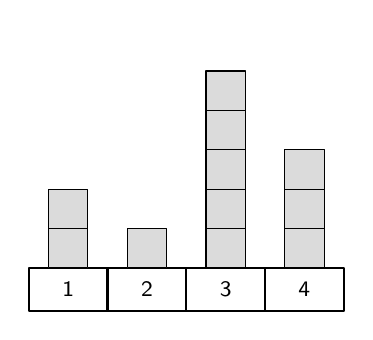
\begin{tikzpicture}[x=1mm,y=1mm,line join=round]
\path (0,0) rectangle (40,36.0);
\draw[thick, fill=white] (0,0) rectangle (10,5.5);
\node[font=\footnotesize] at (5.0,2.75) {1};
\draw[fill=black!14] (2.5,5.5) rectangle (7.5,10.5);
\draw[fill=black!14] (2.5,10.5) rectangle (7.5,15.5);
\draw[thick, fill=white] (10,0) rectangle (20,5.5);
\node[font=\footnotesize] at (15.0,2.75) {2};
\draw[fill=black!14] (12.5,5.5) rectangle (17.5,10.5);
\draw[thick, fill=white] (20,0) rectangle (30,5.5);
\node[font=\footnotesize] at (25.0,2.75) {3};
\draw[fill=black!14] (22.5,5.5) rectangle (27.5,10.5);
\draw[fill=black!14] (22.5,10.5) rectangle (27.5,15.5);
\draw[fill=black!14] (22.5,15.5) rectangle (27.5,20.5);
\draw[fill=black!14] (22.5,20.5) rectangle (27.5,25.5);
\draw[fill=black!14] (22.5,25.5) rectangle (27.5,30.5);
\draw[thick, fill=white] (30,0) rectangle (40,5.5);
\node[font=\footnotesize] at (35.0,2.75) {4};
\draw[fill=black!14] (32.5,5.5) rectangle (37.5,10.5);
\draw[fill=black!14] (32.5,10.5) rectangle (37.5,15.5);
\draw[fill=black!14] (32.5,15.5) rectangle (37.5,20.5);
\end{tikzpicture}\end{minipage}\hfill\begin{minipage}[b]{0.24\linewidth}\centering 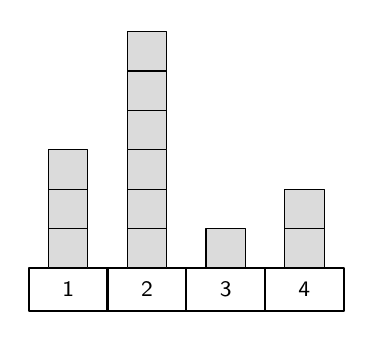
\begin{tikzpicture}[x=1mm,y=1mm,line join=round]
\path (0,0) rectangle (40,36.0);
\draw[thick, fill=white] (0,0) rectangle (10,5.5);
\node[font=\footnotesize] at (5.0,2.75) {1};
\draw[fill=black!14] (2.5,5.5) rectangle (7.5,10.5);
\draw[fill=black!14] (2.5,10.5) rectangle (7.5,15.5);
\draw[fill=black!14] (2.5,15.5) rectangle (7.5,20.5);
\draw[thick, fill=white] (10,0) rectangle (20,5.5);
\node[font=\footnotesize] at (15.0,2.75) {2};
\draw[fill=black!14] (12.5,5.5) rectangle (17.5,10.5);
\draw[fill=black!14] (12.5,10.5) rectangle (17.5,15.5);
\draw[fill=black!14] (12.5,15.5) rectangle (17.5,20.5);
\draw[fill=black!14] (12.5,20.5) rectangle (17.5,25.5);
\draw[fill=black!14] (12.5,25.5) rectangle (17.5,30.5);
\draw[fill=black!14] (12.5,30.5) rectangle (17.5,35.5);
\draw[thick, fill=white] (20,0) rectangle (30,5.5);
\node[font=\footnotesize] at (25.0,2.75) {3};
\draw[fill=black!14] (22.5,5.5) rectangle (27.5,10.5);
\draw[thick, fill=white] (30,0) rectangle (40,5.5);
\node[font=\footnotesize] at (35.0,2.75) {4};
\draw[fill=black!14] (32.5,5.5) rectangle (37.5,10.5);
\draw[fill=black!14] (32.5,10.5) rectangle (37.5,15.5);
\end{tikzpicture}\end{minipage}\hfill\begin{minipage}[b]{0.24\linewidth}\centering 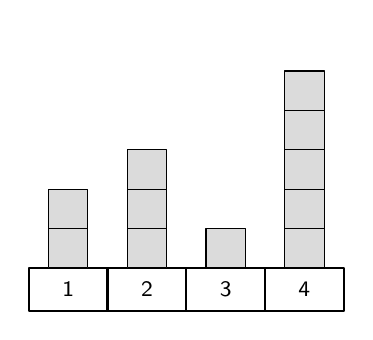
\begin{tikzpicture}[x=1mm,y=1mm,line join=round]
\path (0,0) rectangle (40,36.0);
\draw[thick, fill=white] (0,0) rectangle (10,5.5);
\node[font=\footnotesize] at (5.0,2.75) {1};
\draw[fill=black!14] (2.5,5.5) rectangle (7.5,10.5);
\draw[fill=black!14] (2.5,10.5) rectangle (7.5,15.5);
\draw[thick, fill=white] (10,0) rectangle (20,5.5);
\node[font=\footnotesize] at (15.0,2.75) {2};
\draw[fill=black!14] (12.5,5.5) rectangle (17.5,10.5);
\draw[fill=black!14] (12.5,10.5) rectangle (17.5,15.5);
\draw[fill=black!14] (12.5,15.5) rectangle (17.5,20.5);
\draw[thick, fill=white] (20,0) rectangle (30,5.5);
\node[font=\footnotesize] at (25.0,2.75) {3};
\draw[fill=black!14] (22.5,5.5) rectangle (27.5,10.5);
\draw[thick, fill=white] (30,0) rectangle (40,5.5);
\node[font=\footnotesize] at (35.0,2.75) {4};
\draw[fill=black!14] (32.5,5.5) rectangle (37.5,10.5);
\draw[fill=black!14] (32.5,10.5) rectangle (37.5,15.5);
\draw[fill=black!14] (32.5,15.5) rectangle (37.5,20.5);
\draw[fill=black!14] (32.5,20.5) rectangle (37.5,25.5);
\draw[fill=black!14] (32.5,25.5) rectangle (37.5,30.5);
\end{tikzpicture}\end{minipage}\hfill\begin{minipage}[b]{0.24\linewidth}\centering 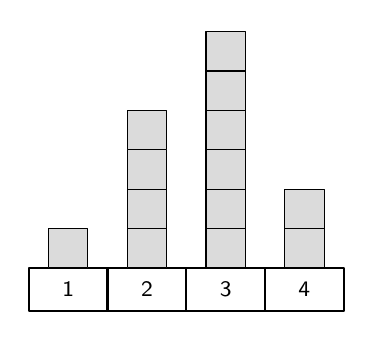
\begin{tikzpicture}[x=1mm,y=1mm,line join=round]
\path (0,0) rectangle (40,36.0);
\draw[thick, fill=white] (0,0) rectangle (10,5.5);
\node[font=\footnotesize] at (5.0,2.75) {1};
\draw[fill=black!14] (2.5,5.5) rectangle (7.5,10.5);
\draw[thick, fill=white] (10,0) rectangle (20,5.5);
\node[font=\footnotesize] at (15.0,2.75) {2};
\draw[fill=black!14] (12.5,5.5) rectangle (17.5,10.5);
\draw[fill=black!14] (12.5,10.5) rectangle (17.5,15.5);
\draw[fill=black!14] (12.5,15.5) rectangle (17.5,20.5);
\draw[fill=black!14] (12.5,20.5) rectangle (17.5,25.5);
\draw[thick, fill=white] (20,0) rectangle (30,5.5);
\node[font=\footnotesize] at (25.0,2.75) {3};
\draw[fill=black!14] (22.5,5.5) rectangle (27.5,10.5);
\draw[fill=black!14] (22.5,10.5) rectangle (27.5,15.5);
\draw[fill=black!14] (22.5,15.5) rectangle (27.5,20.5);
\draw[fill=black!14] (22.5,20.5) rectangle (27.5,25.5);
\draw[fill=black!14] (22.5,25.5) rectangle (27.5,30.5);
\draw[fill=black!14] (22.5,30.5) rectangle (27.5,35.5);
\draw[thick, fill=white] (30,0) rectangle (40,5.5);
\node[font=\footnotesize] at (35.0,2.75) {4};
\draw[fill=black!14] (32.5,5.5) rectangle (37.5,10.5);
\draw[fill=black!14] (32.5,10.5) rectangle (37.5,15.5);
\end{tikzpicture}\end{minipage}\par\vspace{2mm}\problem Is it better to go first or second on each of these rows? Ring your answer. Then find a way to tell from the three heights, without playing.\par\vspace{4mm}\noindent \begin{minipage}[b]{0.32\linewidth}\centering 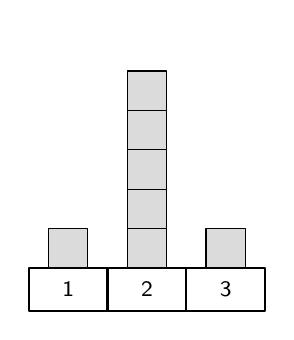
\begin{tikzpicture}[x=1mm,y=1mm,line join=round]
\path (0,0) rectangle (30,36.0);
\draw[thick, fill=white] (0,0) rectangle (10,5.5);
\node[font=\footnotesize] at (5.0,2.75) {1};
\draw[fill=black!14] (2.5,5.5) rectangle (7.5,10.5);
\draw[thick, fill=white] (10,0) rectangle (20,5.5);
\node[font=\footnotesize] at (15.0,2.75) {2};
\draw[fill=black!14] (12.5,5.5) rectangle (17.5,10.5);
\draw[fill=black!14] (12.5,10.5) rectangle (17.5,15.5);
\draw[fill=black!14] (12.5,15.5) rectangle (17.5,20.5);
\draw[fill=black!14] (12.5,20.5) rectangle (17.5,25.5);
\draw[fill=black!14] (12.5,25.5) rectangle (17.5,30.5);
\draw[thick, fill=white] (20,0) rectangle (30,5.5);
\node[font=\footnotesize] at (25.0,2.75) {3};
\draw[fill=black!14] (22.5,5.5) rectangle (27.5,10.5);
\end{tikzpicture}\\[2mm]{\small first\hspace{4mm}second\hspace{4mm}no difference}\end{minipage}\hfill\begin{minipage}[b]{0.32\linewidth}\centering 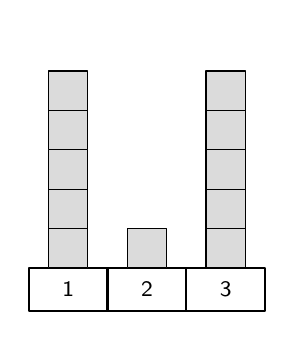
\begin{tikzpicture}[x=1mm,y=1mm,line join=round]
\path (0,0) rectangle (30,36.0);
\draw[thick, fill=white] (0,0) rectangle (10,5.5);
\node[font=\footnotesize] at (5.0,2.75) {1};
\draw[fill=black!14] (2.5,5.5) rectangle (7.5,10.5);
\draw[fill=black!14] (2.5,10.5) rectangle (7.5,15.5);
\draw[fill=black!14] (2.5,15.5) rectangle (7.5,20.5);
\draw[fill=black!14] (2.5,20.5) rectangle (7.5,25.5);
\draw[fill=black!14] (2.5,25.5) rectangle (7.5,30.5);
\draw[thick, fill=white] (10,0) rectangle (20,5.5);
\node[font=\footnotesize] at (15.0,2.75) {2};
\draw[fill=black!14] (12.5,5.5) rectangle (17.5,10.5);
\draw[thick, fill=white] (20,0) rectangle (30,5.5);
\node[font=\footnotesize] at (25.0,2.75) {3};
\draw[fill=black!14] (22.5,5.5) rectangle (27.5,10.5);
\draw[fill=black!14] (22.5,10.5) rectangle (27.5,15.5);
\draw[fill=black!14] (22.5,15.5) rectangle (27.5,20.5);
\draw[fill=black!14] (22.5,20.5) rectangle (27.5,25.5);
\draw[fill=black!14] (22.5,25.5) rectangle (27.5,30.5);
\end{tikzpicture}\\[2mm]{\small first\hspace{4mm}second\hspace{4mm}no difference}\end{minipage}\hfill\begin{minipage}[b]{0.32\linewidth}\centering 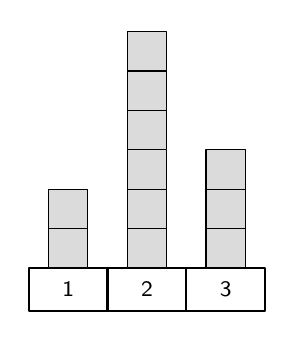
\begin{tikzpicture}[x=1mm,y=1mm,line join=round]
\path (0,0) rectangle (30,36.0);
\draw[thick, fill=white] (0,0) rectangle (10,5.5);
\node[font=\footnotesize] at (5.0,2.75) {1};
\draw[fill=black!14] (2.5,5.5) rectangle (7.5,10.5);
\draw[fill=black!14] (2.5,10.5) rectangle (7.5,15.5);
\draw[thick, fill=white] (10,0) rectangle (20,5.5);
\node[font=\footnotesize] at (15.0,2.75) {2};
\draw[fill=black!14] (12.5,5.5) rectangle (17.5,10.5);
\draw[fill=black!14] (12.5,10.5) rectangle (17.5,15.5);
\draw[fill=black!14] (12.5,15.5) rectangle (17.5,20.5);
\draw[fill=black!14] (12.5,20.5) rectangle (17.5,25.5);
\draw[fill=black!14] (12.5,25.5) rectangle (17.5,30.5);
\draw[fill=black!14] (12.5,30.5) rectangle (17.5,35.5);
\draw[thick, fill=white] (20,0) rectangle (30,5.5);
\node[font=\footnotesize] at (25.0,2.75) {3};
\draw[fill=black!14] (22.5,5.5) rectangle (27.5,10.5);
\draw[fill=black!14] (22.5,10.5) rectangle (27.5,15.5);
\draw[fill=black!14] (22.5,15.5) rectangle (27.5,20.5);
\end{tikzpicture}\\[2mm]{\small first\hspace{4mm}second\hspace{4mm}no difference}\end{minipage}\par\vspace{6mm}
\noindent \begin{minipage}[b]{0.32\linewidth}\centering 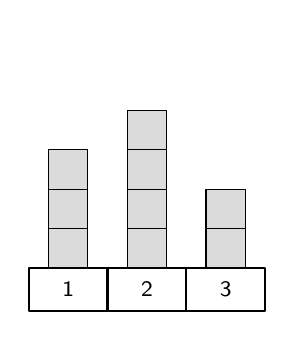
\begin{tikzpicture}[x=1mm,y=1mm,line join=round]
\path (0,0) rectangle (30,36.0);
\draw[thick, fill=white] (0,0) rectangle (10,5.5);
\node[font=\footnotesize] at (5.0,2.75) {1};
\draw[fill=black!14] (2.5,5.5) rectangle (7.5,10.5);
\draw[fill=black!14] (2.5,10.5) rectangle (7.5,15.5);
\draw[fill=black!14] (2.5,15.5) rectangle (7.5,20.5);
\draw[thick, fill=white] (10,0) rectangle (20,5.5);
\node[font=\footnotesize] at (15.0,2.75) {2};
\draw[fill=black!14] (12.5,5.5) rectangle (17.5,10.5);
\draw[fill=black!14] (12.5,10.5) rectangle (17.5,15.5);
\draw[fill=black!14] (12.5,15.5) rectangle (17.5,20.5);
\draw[fill=black!14] (12.5,20.5) rectangle (17.5,25.5);
\draw[thick, fill=white] (20,0) rectangle (30,5.5);
\node[font=\footnotesize] at (25.0,2.75) {3};
\draw[fill=black!14] (22.5,5.5) rectangle (27.5,10.5);
\draw[fill=black!14] (22.5,10.5) rectangle (27.5,15.5);
\end{tikzpicture}\\[2mm]{\small first\hspace{4mm}second\hspace{4mm}no difference}\end{minipage}\hfill\begin{minipage}[b]{0.32\linewidth}\centering 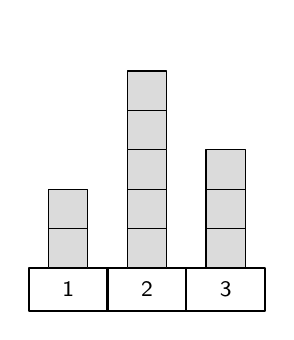
\begin{tikzpicture}[x=1mm,y=1mm,line join=round]
\path (0,0) rectangle (30,36.0);
\draw[thick, fill=white] (0,0) rectangle (10,5.5);
\node[font=\footnotesize] at (5.0,2.75) {1};
\draw[fill=black!14] (2.5,5.5) rectangle (7.5,10.5);
\draw[fill=black!14] (2.5,10.5) rectangle (7.5,15.5);
\draw[thick, fill=white] (10,0) rectangle (20,5.5);
\node[font=\footnotesize] at (15.0,2.75) {2};
\draw[fill=black!14] (12.5,5.5) rectangle (17.5,10.5);
\draw[fill=black!14] (12.5,10.5) rectangle (17.5,15.5);
\draw[fill=black!14] (12.5,15.5) rectangle (17.5,20.5);
\draw[fill=black!14] (12.5,20.5) rectangle (17.5,25.5);
\draw[fill=black!14] (12.5,25.5) rectangle (17.5,30.5);
\draw[thick, fill=white] (20,0) rectangle (30,5.5);
\node[font=\footnotesize] at (25.0,2.75) {3};
\draw[fill=black!14] (22.5,5.5) rectangle (27.5,10.5);
\draw[fill=black!14] (22.5,10.5) rectangle (27.5,15.5);
\draw[fill=black!14] (22.5,15.5) rectangle (27.5,20.5);
\end{tikzpicture}\\[2mm]{\small first\hspace{4mm}second\hspace{4mm}no difference}\end{minipage}\hfill\begin{minipage}[b]{0.32\linewidth}\centering 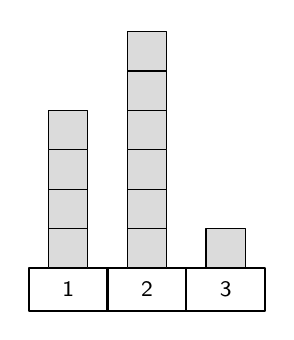
\begin{tikzpicture}[x=1mm,y=1mm,line join=round]
\path (0,0) rectangle (30,36.0);
\draw[thick, fill=white] (0,0) rectangle (10,5.5);
\node[font=\footnotesize] at (5.0,2.75) {1};
\draw[fill=black!14] (2.5,5.5) rectangle (7.5,10.5);
\draw[fill=black!14] (2.5,10.5) rectangle (7.5,15.5);
\draw[fill=black!14] (2.5,15.5) rectangle (7.5,20.5);
\draw[fill=black!14] (2.5,20.5) rectangle (7.5,25.5);
\draw[thick, fill=white] (10,0) rectangle (20,5.5);
\node[font=\footnotesize] at (15.0,2.75) {2};
\draw[fill=black!14] (12.5,5.5) rectangle (17.5,10.5);
\draw[fill=black!14] (12.5,10.5) rectangle (17.5,15.5);
\draw[fill=black!14] (12.5,15.5) rectangle (17.5,20.5);
\draw[fill=black!14] (12.5,20.5) rectangle (17.5,25.5);
\draw[fill=black!14] (12.5,25.5) rectangle (17.5,30.5);
\draw[fill=black!14] (12.5,30.5) rectangle (17.5,35.5);
\draw[thick, fill=white] (20,0) rectangle (30,5.5);
\node[font=\footnotesize] at (25.0,2.75) {3};
\draw[fill=black!14] (22.5,5.5) rectangle (27.5,10.5);
\end{tikzpicture}\\[2mm]{\small first\hspace{4mm}second\hspace{4mm}no difference}\end{minipage}\par\vspace{6mm}\ruledlines{4}{8mm}\newpage\problem Can you find a row of four towers on which the first player loses, however the first player plays?\par\vspace{2mm}\vspace{4mm}\noindent \begin{minipage}[b]{0.48\linewidth}\centering 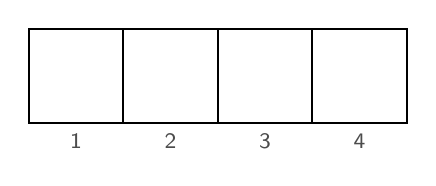
\begin{tikzpicture}[x=1mm,y=1mm]
\draw[thick, fill=white] (0,0) rectangle (12,12);
\node[font=\footnotesize, black!70] at (6.0,-2.3) {1};
\draw[thick, fill=white] (12,0) rectangle (24,12);
\node[font=\footnotesize, black!70] at (18.0,-2.3) {2};
\draw[thick, fill=white] (24,0) rectangle (36,12);
\node[font=\footnotesize, black!70] at (30.0,-2.3) {3};
\draw[thick, fill=white] (36,0) rectangle (48,12);
\node[font=\footnotesize, black!70] at (42.0,-2.3) {4};
\end{tikzpicture}\end{minipage}\hfill\begin{minipage}[b]{0.48\linewidth}\centering 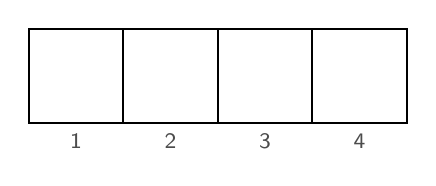
\begin{tikzpicture}[x=1mm,y=1mm]
\draw[thick, fill=white] (0,0) rectangle (12,12);
\node[font=\footnotesize, black!70] at (6.0,-2.3) {1};
\draw[thick, fill=white] (12,0) rectangle (24,12);
\node[font=\footnotesize, black!70] at (18.0,-2.3) {2};
\draw[thick, fill=white] (24,0) rectangle (36,12);
\node[font=\footnotesize, black!70] at (30.0,-2.3) {3};
\draw[thick, fill=white] (36,0) rectangle (48,12);
\node[font=\footnotesize, black!70] at (42.0,-2.3) {4};
\end{tikzpicture}\end{minipage}\par\vspace{9mm}
\noindent \begin{minipage}[b]{0.48\linewidth}\centering 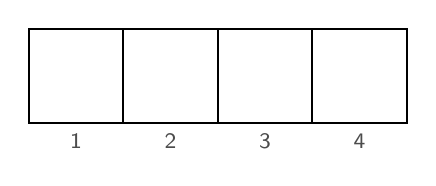
\begin{tikzpicture}[x=1mm,y=1mm]
\draw[thick, fill=white] (0,0) rectangle (12,12);
\node[font=\footnotesize, black!70] at (6.0,-2.3) {1};
\draw[thick, fill=white] (12,0) rectangle (24,12);
\node[font=\footnotesize, black!70] at (18.0,-2.3) {2};
\draw[thick, fill=white] (24,0) rectangle (36,12);
\node[font=\footnotesize, black!70] at (30.0,-2.3) {3};
\draw[thick, fill=white] (36,0) rectangle (48,12);
\node[font=\footnotesize, black!70] at (42.0,-2.3) {4};
\end{tikzpicture}\end{minipage}\hfill\begin{minipage}[b]{0.48\linewidth}\centering 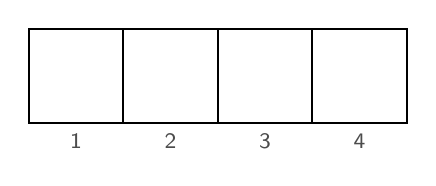
\begin{tikzpicture}[x=1mm,y=1mm]
\draw[thick, fill=white] (0,0) rectangle (12,12);
\node[font=\footnotesize, black!70] at (6.0,-2.3) {1};
\draw[thick, fill=white] (12,0) rectangle (24,12);
\node[font=\footnotesize, black!70] at (18.0,-2.3) {2};
\draw[thick, fill=white] (24,0) rectangle (36,12);
\node[font=\footnotesize, black!70] at (30.0,-2.3) {3};
\draw[thick, fill=white] (36,0) rectangle (48,12);
\node[font=\footnotesize, black!70] at (42.0,-2.3) {4};
\end{tikzpicture}\end{minipage}\par\vspace{9mm}
\noindent \begin{minipage}[b]{0.48\linewidth}\centering 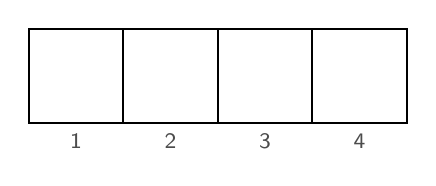
\begin{tikzpicture}[x=1mm,y=1mm]
\draw[thick, fill=white] (0,0) rectangle (12,12);
\node[font=\footnotesize, black!70] at (6.0,-2.3) {1};
\draw[thick, fill=white] (12,0) rectangle (24,12);
\node[font=\footnotesize, black!70] at (18.0,-2.3) {2};
\draw[thick, fill=white] (24,0) rectangle (36,12);
\node[font=\footnotesize, black!70] at (30.0,-2.3) {3};
\draw[thick, fill=white] (36,0) rectangle (48,12);
\node[font=\footnotesize, black!70] at (42.0,-2.3) {4};
\end{tikzpicture}\end{minipage}\hfill\begin{minipage}[b]{0.48\linewidth}\centering 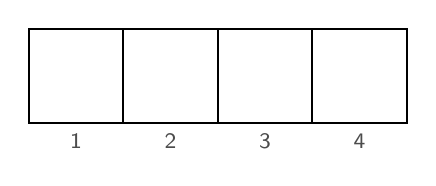
\begin{tikzpicture}[x=1mm,y=1mm]
\draw[thick, fill=white] (0,0) rectangle (12,12);
\node[font=\footnotesize, black!70] at (6.0,-2.3) {1};
\draw[thick, fill=white] (12,0) rectangle (24,12);
\node[font=\footnotesize, black!70] at (18.0,-2.3) {2};
\draw[thick, fill=white] (24,0) rectangle (36,12);
\node[font=\footnotesize, black!70] at (30.0,-2.3) {3};
\draw[thick, fill=white] (36,0) rectangle (48,12);
\node[font=\footnotesize, black!70] at (42.0,-2.3) {4};
\end{tikzpicture}\end{minipage}\par\vspace{9mm}
\noindent \begin{minipage}[b]{0.48\linewidth}\centering 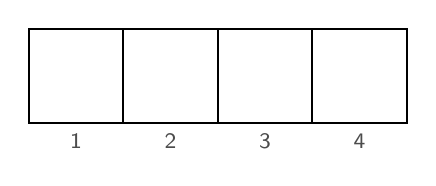
\begin{tikzpicture}[x=1mm,y=1mm]
\draw[thick, fill=white] (0,0) rectangle (12,12);
\node[font=\footnotesize, black!70] at (6.0,-2.3) {1};
\draw[thick, fill=white] (12,0) rectangle (24,12);
\node[font=\footnotesize, black!70] at (18.0,-2.3) {2};
\draw[thick, fill=white] (24,0) rectangle (36,12);
\node[font=\footnotesize, black!70] at (30.0,-2.3) {3};
\draw[thick, fill=white] (36,0) rectangle (48,12);
\node[font=\footnotesize, black!70] at (42.0,-2.3) {4};
\end{tikzpicture}\end{minipage}\hfill\begin{minipage}[b]{0.48\linewidth}\centering 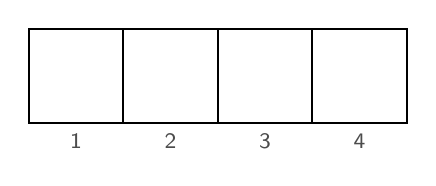
\begin{tikzpicture}[x=1mm,y=1mm]
\draw[thick, fill=white] (0,0) rectangle (12,12);
\node[font=\footnotesize, black!70] at (6.0,-2.3) {1};
\draw[thick, fill=white] (12,0) rectangle (24,12);
\node[font=\footnotesize, black!70] at (18.0,-2.3) {2};
\draw[thick, fill=white] (24,0) rectangle (36,12);
\node[font=\footnotesize, black!70] at (30.0,-2.3) {3};
\draw[thick, fill=white] (36,0) rectangle (48,12);
\node[font=\footnotesize, black!70] at (42.0,-2.3) {4};
\end{tikzpicture}\end{minipage}\par\vspace{9mm}\ruledlines{5}{9mm}\newpage\problem You and your partner play the grown-up together. The grown-up goes first on these colored rows. Can you beat the grown-up? How does the grown-up choose which towers to take?\par\vspace{4mm}\noindent \begin{minipage}[b]{0.48\linewidth}\centering 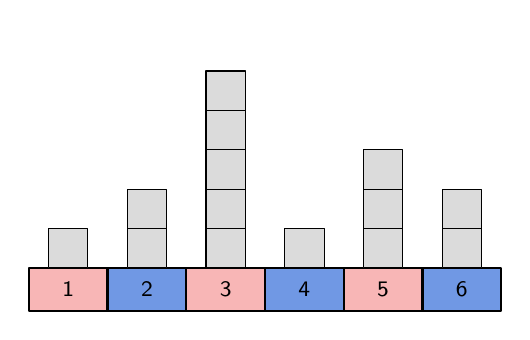
\begin{tikzpicture}[x=1mm,y=1mm,line join=round]
\path (0,0) rectangle (60,36.0);
\draw[thick, fill=slotred] (0,0) rectangle (10,5.5);
\node[font=\footnotesize] at (5.0,2.75) {1};
\draw[fill=black!14] (2.5,5.5) rectangle (7.5,10.5);
\draw[thick, fill=slotblue] (10,0) rectangle (20,5.5);
\node[font=\footnotesize] at (15.0,2.75) {2};
\draw[fill=black!14] (12.5,5.5) rectangle (17.5,10.5);
\draw[fill=black!14] (12.5,10.5) rectangle (17.5,15.5);
\draw[thick, fill=slotred] (20,0) rectangle (30,5.5);
\node[font=\footnotesize] at (25.0,2.75) {3};
\draw[fill=black!14] (22.5,5.5) rectangle (27.5,10.5);
\draw[fill=black!14] (22.5,10.5) rectangle (27.5,15.5);
\draw[fill=black!14] (22.5,15.5) rectangle (27.5,20.5);
\draw[fill=black!14] (22.5,20.5) rectangle (27.5,25.5);
\draw[fill=black!14] (22.5,25.5) rectangle (27.5,30.5);
\draw[thick, fill=slotblue] (30,0) rectangle (40,5.5);
\node[font=\footnotesize] at (35.0,2.75) {4};
\draw[fill=black!14] (32.5,5.5) rectangle (37.5,10.5);
\draw[thick, fill=slotred] (40,0) rectangle (50,5.5);
\node[font=\footnotesize] at (45.0,2.75) {5};
\draw[fill=black!14] (42.5,5.5) rectangle (47.5,10.5);
\draw[fill=black!14] (42.5,10.5) rectangle (47.5,15.5);
\draw[fill=black!14] (42.5,15.5) rectangle (47.5,20.5);
\draw[thick, fill=slotblue] (50,0) rectangle (60,5.5);
\node[font=\footnotesize] at (55.0,2.75) {6};
\draw[fill=black!14] (52.5,5.5) rectangle (57.5,10.5);
\draw[fill=black!14] (52.5,10.5) rectangle (57.5,15.5);
\end{tikzpicture}\end{minipage}\hfill\begin{minipage}[b]{0.48\linewidth}\centering 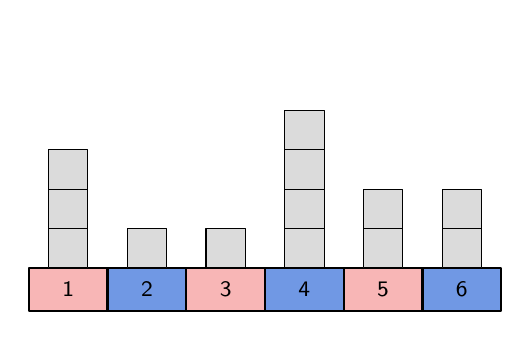
\begin{tikzpicture}[x=1mm,y=1mm,line join=round]
\path (0,0) rectangle (60,36.0);
\draw[thick, fill=slotred] (0,0) rectangle (10,5.5);
\node[font=\footnotesize] at (5.0,2.75) {1};
\draw[fill=black!14] (2.5,5.5) rectangle (7.5,10.5);
\draw[fill=black!14] (2.5,10.5) rectangle (7.5,15.5);
\draw[fill=black!14] (2.5,15.5) rectangle (7.5,20.5);
\draw[thick, fill=slotblue] (10,0) rectangle (20,5.5);
\node[font=\footnotesize] at (15.0,2.75) {2};
\draw[fill=black!14] (12.5,5.5) rectangle (17.5,10.5);
\draw[thick, fill=slotred] (20,0) rectangle (30,5.5);
\node[font=\footnotesize] at (25.0,2.75) {3};
\draw[fill=black!14] (22.5,5.5) rectangle (27.5,10.5);
\draw[thick, fill=slotblue] (30,0) rectangle (40,5.5);
\node[font=\footnotesize] at (35.0,2.75) {4};
\draw[fill=black!14] (32.5,5.5) rectangle (37.5,10.5);
\draw[fill=black!14] (32.5,10.5) rectangle (37.5,15.5);
\draw[fill=black!14] (32.5,15.5) rectangle (37.5,20.5);
\draw[fill=black!14] (32.5,20.5) rectangle (37.5,25.5);
\draw[thick, fill=slotred] (40,0) rectangle (50,5.5);
\node[font=\footnotesize] at (45.0,2.75) {5};
\draw[fill=black!14] (42.5,5.5) rectangle (47.5,10.5);
\draw[fill=black!14] (42.5,10.5) rectangle (47.5,15.5);
\draw[thick, fill=slotblue] (50,0) rectangle (60,5.5);
\node[font=\footnotesize] at (55.0,2.75) {6};
\draw[fill=black!14] (52.5,5.5) rectangle (57.5,10.5);
\draw[fill=black!14] (52.5,10.5) rectangle (57.5,15.5);
\end{tikzpicture}\end{minipage}\par\vspace{5mm}\centerline{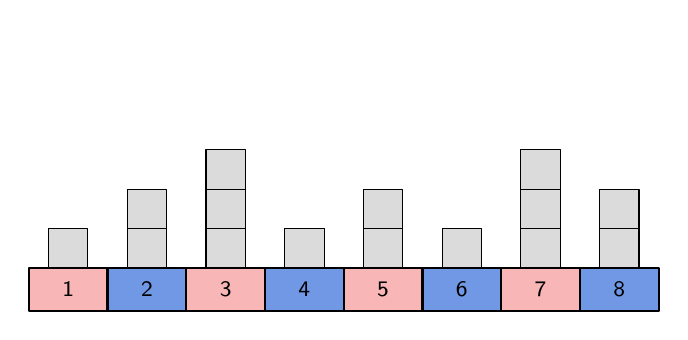
\begin{tikzpicture}[x=1mm,y=1mm,line join=round]
\path (0,0) rectangle (80,36.0);
\draw[thick, fill=slotred] (0,0) rectangle (10,5.5);
\node[font=\footnotesize] at (5.0,2.75) {1};
\draw[fill=black!14] (2.5,5.5) rectangle (7.5,10.5);
\draw[thick, fill=slotblue] (10,0) rectangle (20,5.5);
\node[font=\footnotesize] at (15.0,2.75) {2};
\draw[fill=black!14] (12.5,5.5) rectangle (17.5,10.5);
\draw[fill=black!14] (12.5,10.5) rectangle (17.5,15.5);
\draw[thick, fill=slotred] (20,0) rectangle (30,5.5);
\node[font=\footnotesize] at (25.0,2.75) {3};
\draw[fill=black!14] (22.5,5.5) rectangle (27.5,10.5);
\draw[fill=black!14] (22.5,10.5) rectangle (27.5,15.5);
\draw[fill=black!14] (22.5,15.5) rectangle (27.5,20.5);
\draw[thick, fill=slotblue] (30,0) rectangle (40,5.5);
\node[font=\footnotesize] at (35.0,2.75) {4};
\draw[fill=black!14] (32.5,5.5) rectangle (37.5,10.5);
\draw[thick, fill=slotred] (40,0) rectangle (50,5.5);
\node[font=\footnotesize] at (45.0,2.75) {5};
\draw[fill=black!14] (42.5,5.5) rectangle (47.5,10.5);
\draw[fill=black!14] (42.5,10.5) rectangle (47.5,15.5);
\draw[thick, fill=slotblue] (50,0) rectangle (60,5.5);
\node[font=\footnotesize] at (55.0,2.75) {6};
\draw[fill=black!14] (52.5,5.5) rectangle (57.5,10.5);
\draw[thick, fill=slotred] (60,0) rectangle (70,5.5);
\node[font=\footnotesize] at (65.0,2.75) {7};
\draw[fill=black!14] (62.5,5.5) rectangle (67.5,10.5);
\draw[fill=black!14] (62.5,10.5) rectangle (67.5,15.5);
\draw[fill=black!14] (62.5,15.5) rectangle (67.5,20.5);
\draw[thick, fill=slotblue] (70,0) rectangle (80,5.5);
\node[font=\footnotesize] at (75.0,2.75) {8};
\draw[fill=black!14] (72.5,5.5) rectangle (77.5,10.5);
\draw[fill=black!14] (72.5,10.5) rectangle (77.5,15.5);
\end{tikzpicture}}\par\ruledlines{6}{8mm}\newpage\problem Go first on this colored row using the grown-up's plan. Can your partner ever make you take a tower on the other color? Try every way your partner can play, and write each game as the slot numbers in the order the towers were taken.\par\vspace{4mm}\centerline{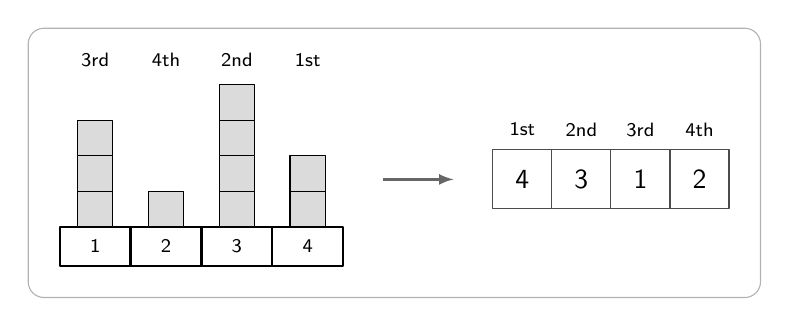
\begin{tikzpicture}[x=1mm,y=1mm,line join=round]
\draw[thick, fill=white] (0.0,0) rectangle (9.0,5.0);
\node[font=\scriptsize] at (4.5,2.5) {1};
\draw[fill=black!14] (2.25,5.0) rectangle (6.75,9.5);
\draw[fill=black!14] (2.25,9.5) rectangle (6.75,14.0);
\draw[fill=black!14] (2.25,14.0) rectangle (6.75,18.5);
\node[font=\scriptsize] at (4.5,26.2) {3rd};
\draw[thick, fill=white] (9.0,0) rectangle (18.0,5.0);
\node[font=\scriptsize] at (13.5,2.5) {2};
\draw[fill=black!14] (11.25,5.0) rectangle (15.75,9.5);
\node[font=\scriptsize] at (13.5,26.2) {4th};
\draw[thick, fill=white] (18.0,0) rectangle (27.0,5.0);
\node[font=\scriptsize] at (22.5,2.5) {3};
\draw[fill=black!14] (20.25,5.0) rectangle (24.75,9.5);
\draw[fill=black!14] (20.25,9.5) rectangle (24.75,14.0);
\draw[fill=black!14] (20.25,14.0) rectangle (24.75,18.5);
\draw[fill=black!14] (20.25,18.5) rectangle (24.75,23.0);
\node[font=\scriptsize] at (22.5,26.2) {2nd};
\draw[thick, fill=white] (27.0,0) rectangle (36.0,5.0);
\node[font=\scriptsize] at (31.5,2.5) {4};
\draw[fill=black!14] (29.25,5.0) rectangle (33.75,9.5);
\draw[fill=black!14] (29.25,9.5) rectangle (33.75,14.0);
\node[font=\scriptsize] at (31.5,26.2) {1st};
\draw[-latex, black!60, thick] (41.0,11.0) -- (50.0,11.0);
\draw[black!70] (55.0,7.25) rectangle (62.5,14.75);
\node[font=\normalsize] at (58.75,11.0) {4};
\node[font=\scriptsize] at (58.75,17.35) {1st};
\draw[black!70] (62.5,7.25) rectangle (70.0,14.75);
\node[font=\normalsize] at (66.25,11.0) {3};
\node[font=\scriptsize] at (66.25,17.35) {2nd};
\draw[black!70] (70.0,7.25) rectangle (77.5,14.75);
\node[font=\normalsize] at (73.75,11.0) {1};
\node[font=\scriptsize] at (73.75,17.35) {3rd};
\draw[black!70] (77.5,7.25) rectangle (85.0,14.75);
\node[font=\normalsize] at (81.25,11.0) {2};
\node[font=\scriptsize] at (81.25,17.35) {4th};
\draw[black!30, rounded corners=2mm] (-4,-4) rectangle (89.0,30.2);
\end{tikzpicture}}\par\vspace{7mm}\centerline{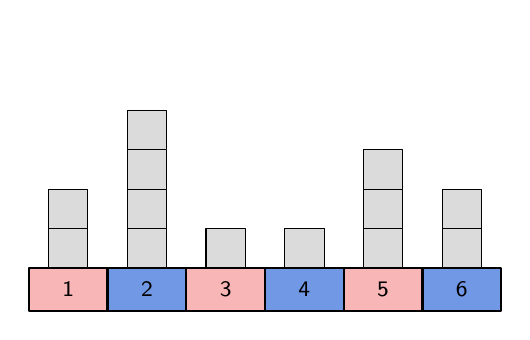
\begin{tikzpicture}[x=1mm,y=1mm,line join=round]
\path (0,0) rectangle (60,36.0);
\draw[thick, fill=slotred] (0,0) rectangle (10,5.5);
\node[font=\footnotesize] at (5.0,2.75) {1};
\draw[fill=black!14] (2.5,5.5) rectangle (7.5,10.5);
\draw[fill=black!14] (2.5,10.5) rectangle (7.5,15.5);
\draw[thick, fill=slotblue] (10,0) rectangle (20,5.5);
\node[font=\footnotesize] at (15.0,2.75) {2};
\draw[fill=black!14] (12.5,5.5) rectangle (17.5,10.5);
\draw[fill=black!14] (12.5,10.5) rectangle (17.5,15.5);
\draw[fill=black!14] (12.5,15.5) rectangle (17.5,20.5);
\draw[fill=black!14] (12.5,20.5) rectangle (17.5,25.5);
\draw[thick, fill=slotred] (20,0) rectangle (30,5.5);
\node[font=\footnotesize] at (25.0,2.75) {3};
\draw[fill=black!14] (22.5,5.5) rectangle (27.5,10.5);
\draw[thick, fill=slotblue] (30,0) rectangle (40,5.5);
\node[font=\footnotesize] at (35.0,2.75) {4};
\draw[fill=black!14] (32.5,5.5) rectangle (37.5,10.5);
\draw[thick, fill=slotred] (40,0) rectangle (50,5.5);
\node[font=\footnotesize] at (45.0,2.75) {5};
\draw[fill=black!14] (42.5,5.5) rectangle (47.5,10.5);
\draw[fill=black!14] (42.5,10.5) rectangle (47.5,15.5);
\draw[fill=black!14] (42.5,15.5) rectangle (47.5,20.5);
\draw[thick, fill=slotblue] (50,0) rectangle (60,5.5);
\node[font=\footnotesize] at (55.0,2.75) {6};
\draw[fill=black!14] (52.5,5.5) rectangle (57.5,10.5);
\draw[fill=black!14] (52.5,10.5) rectangle (57.5,15.5);
\end{tikzpicture}}\par\vspace{6mm}\noindent\hfill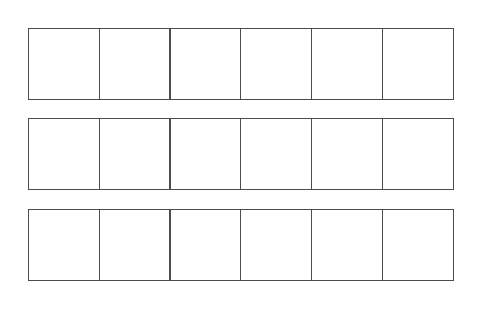
\begin{tikzpicture}[x=1mm,y=1mm]
\draw[black!70] (0.0,0.0) rectangle (9.0,9.0);
\draw[black!70] (9.0,0.0) rectangle (18.0,9.0);
\draw[black!70] (18.0,0.0) rectangle (27.0,9.0);
\draw[black!70] (27.0,0.0) rectangle (36.0,9.0);
\draw[black!70] (36.0,0.0) rectangle (45.0,9.0);
\draw[black!70] (45.0,0.0) rectangle (54.0,9.0);
\draw[black!70] (0.0,-11.5) rectangle (9.0,-2.5);
\draw[black!70] (9.0,-11.5) rectangle (18.0,-2.5);
\draw[black!70] (18.0,-11.5) rectangle (27.0,-2.5);
\draw[black!70] (27.0,-11.5) rectangle (36.0,-2.5);
\draw[black!70] (36.0,-11.5) rectangle (45.0,-2.5);
\draw[black!70] (45.0,-11.5) rectangle (54.0,-2.5);
\draw[black!70] (0.0,-23.0) rectangle (9.0,-14.0);
\draw[black!70] (9.0,-23.0) rectangle (18.0,-14.0);
\draw[black!70] (18.0,-23.0) rectangle (27.0,-14.0);
\draw[black!70] (27.0,-23.0) rectangle (36.0,-14.0);
\draw[black!70] (36.0,-23.0) rectangle (45.0,-14.0);
\draw[black!70] (45.0,-23.0) rectangle (54.0,-14.0);
\end{tikzpicture}\hfill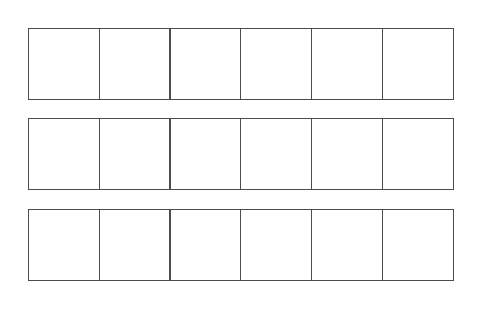
\begin{tikzpicture}[x=1mm,y=1mm]
\draw[black!70] (0.0,0.0) rectangle (9.0,9.0);
\draw[black!70] (9.0,0.0) rectangle (18.0,9.0);
\draw[black!70] (18.0,0.0) rectangle (27.0,9.0);
\draw[black!70] (27.0,0.0) rectangle (36.0,9.0);
\draw[black!70] (36.0,0.0) rectangle (45.0,9.0);
\draw[black!70] (45.0,0.0) rectangle (54.0,9.0);
\draw[black!70] (0.0,-11.5) rectangle (9.0,-2.5);
\draw[black!70] (9.0,-11.5) rectangle (18.0,-2.5);
\draw[black!70] (18.0,-11.5) rectangle (27.0,-2.5);
\draw[black!70] (27.0,-11.5) rectangle (36.0,-2.5);
\draw[black!70] (36.0,-11.5) rectangle (45.0,-2.5);
\draw[black!70] (45.0,-11.5) rectangle (54.0,-2.5);
\draw[black!70] (0.0,-23.0) rectangle (9.0,-14.0);
\draw[black!70] (9.0,-23.0) rectangle (18.0,-14.0);
\draw[black!70] (18.0,-23.0) rectangle (27.0,-14.0);
\draw[black!70] (27.0,-23.0) rectangle (36.0,-14.0);
\draw[black!70] (36.0,-23.0) rectangle (45.0,-14.0);
\draw[black!70] (45.0,-23.0) rectangle (54.0,-14.0);
\end{tikzpicture}\hfill\null\par\newpage\problem In each of these colored rows, the red slots and the blue slots hold the same number of cubes. Which rows can the first player win? Write the totals when both players play as well as they can.\par\vspace{4mm}\noindent \begin{minipage}[b]{0.48\linewidth}\centering 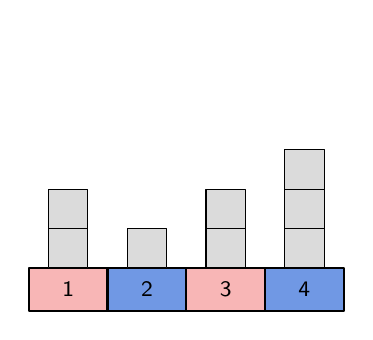
\begin{tikzpicture}[x=1mm,y=1mm,line join=round]
\path (0,0) rectangle (40,36.0);
\draw[thick, fill=slotred] (0,0) rectangle (10,5.5);
\node[font=\footnotesize] at (5.0,2.75) {1};
\draw[fill=black!14] (2.5,5.5) rectangle (7.5,10.5);
\draw[fill=black!14] (2.5,10.5) rectangle (7.5,15.5);
\draw[thick, fill=slotblue] (10,0) rectangle (20,5.5);
\node[font=\footnotesize] at (15.0,2.75) {2};
\draw[fill=black!14] (12.5,5.5) rectangle (17.5,10.5);
\draw[thick, fill=slotred] (20,0) rectangle (30,5.5);
\node[font=\footnotesize] at (25.0,2.75) {3};
\draw[fill=black!14] (22.5,5.5) rectangle (27.5,10.5);
\draw[fill=black!14] (22.5,10.5) rectangle (27.5,15.5);
\draw[thick, fill=slotblue] (30,0) rectangle (40,5.5);
\node[font=\footnotesize] at (35.0,2.75) {4};
\draw[fill=black!14] (32.5,5.5) rectangle (37.5,10.5);
\draw[fill=black!14] (32.5,10.5) rectangle (37.5,15.5);
\draw[fill=black!14] (32.5,15.5) rectangle (37.5,20.5);
\end{tikzpicture}\\[2mm]{\small first \rule{11mm}{0.4pt}\quad second \rule{11mm}{0.4pt}}\end{minipage}\hfill\begin{minipage}[b]{0.48\linewidth}\centering 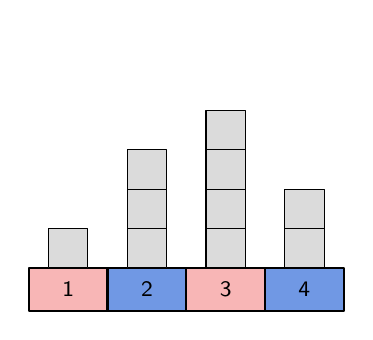
\begin{tikzpicture}[x=1mm,y=1mm,line join=round]
\path (0,0) rectangle (40,36.0);
\draw[thick, fill=slotred] (0,0) rectangle (10,5.5);
\node[font=\footnotesize] at (5.0,2.75) {1};
\draw[fill=black!14] (2.5,5.5) rectangle (7.5,10.5);
\draw[thick, fill=slotblue] (10,0) rectangle (20,5.5);
\node[font=\footnotesize] at (15.0,2.75) {2};
\draw[fill=black!14] (12.5,5.5) rectangle (17.5,10.5);
\draw[fill=black!14] (12.5,10.5) rectangle (17.5,15.5);
\draw[fill=black!14] (12.5,15.5) rectangle (17.5,20.5);
\draw[thick, fill=slotred] (20,0) rectangle (30,5.5);
\node[font=\footnotesize] at (25.0,2.75) {3};
\draw[fill=black!14] (22.5,5.5) rectangle (27.5,10.5);
\draw[fill=black!14] (22.5,10.5) rectangle (27.5,15.5);
\draw[fill=black!14] (22.5,15.5) rectangle (27.5,20.5);
\draw[fill=black!14] (22.5,20.5) rectangle (27.5,25.5);
\draw[thick, fill=slotblue] (30,0) rectangle (40,5.5);
\node[font=\footnotesize] at (35.0,2.75) {4};
\draw[fill=black!14] (32.5,5.5) rectangle (37.5,10.5);
\draw[fill=black!14] (32.5,10.5) rectangle (37.5,15.5);
\end{tikzpicture}\\[2mm]{\small first \rule{11mm}{0.4pt}\quad second \rule{11mm}{0.4pt}}\end{minipage}\par\vspace{7mm}
\noindent \begin{minipage}[b]{0.48\linewidth}\centering 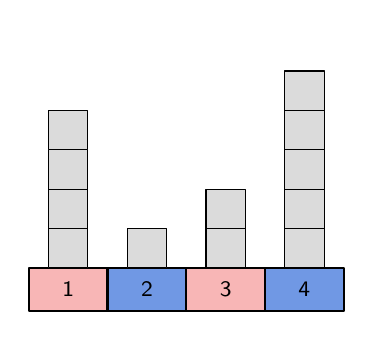
\begin{tikzpicture}[x=1mm,y=1mm,line join=round]
\path (0,0) rectangle (40,36.0);
\draw[thick, fill=slotred] (0,0) rectangle (10,5.5);
\node[font=\footnotesize] at (5.0,2.75) {1};
\draw[fill=black!14] (2.5,5.5) rectangle (7.5,10.5);
\draw[fill=black!14] (2.5,10.5) rectangle (7.5,15.5);
\draw[fill=black!14] (2.5,15.5) rectangle (7.5,20.5);
\draw[fill=black!14] (2.5,20.5) rectangle (7.5,25.5);
\draw[thick, fill=slotblue] (10,0) rectangle (20,5.5);
\node[font=\footnotesize] at (15.0,2.75) {2};
\draw[fill=black!14] (12.5,5.5) rectangle (17.5,10.5);
\draw[thick, fill=slotred] (20,0) rectangle (30,5.5);
\node[font=\footnotesize] at (25.0,2.75) {3};
\draw[fill=black!14] (22.5,5.5) rectangle (27.5,10.5);
\draw[fill=black!14] (22.5,10.5) rectangle (27.5,15.5);
\draw[thick, fill=slotblue] (30,0) rectangle (40,5.5);
\node[font=\footnotesize] at (35.0,2.75) {4};
\draw[fill=black!14] (32.5,5.5) rectangle (37.5,10.5);
\draw[fill=black!14] (32.5,10.5) rectangle (37.5,15.5);
\draw[fill=black!14] (32.5,15.5) rectangle (37.5,20.5);
\draw[fill=black!14] (32.5,20.5) rectangle (37.5,25.5);
\draw[fill=black!14] (32.5,25.5) rectangle (37.5,30.5);
\end{tikzpicture}\\[2mm]{\small first \rule{11mm}{0.4pt}\quad second \rule{11mm}{0.4pt}}\end{minipage}\hfill\begin{minipage}[b]{0.48\linewidth}\centering 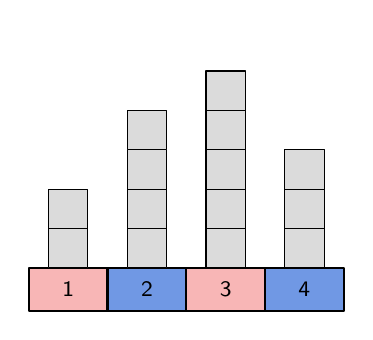
\begin{tikzpicture}[x=1mm,y=1mm,line join=round]
\path (0,0) rectangle (40,36.0);
\draw[thick, fill=slotred] (0,0) rectangle (10,5.5);
\node[font=\footnotesize] at (5.0,2.75) {1};
\draw[fill=black!14] (2.5,5.5) rectangle (7.5,10.5);
\draw[fill=black!14] (2.5,10.5) rectangle (7.5,15.5);
\draw[thick, fill=slotblue] (10,0) rectangle (20,5.5);
\node[font=\footnotesize] at (15.0,2.75) {2};
\draw[fill=black!14] (12.5,5.5) rectangle (17.5,10.5);
\draw[fill=black!14] (12.5,10.5) rectangle (17.5,15.5);
\draw[fill=black!14] (12.5,15.5) rectangle (17.5,20.5);
\draw[fill=black!14] (12.5,20.5) rectangle (17.5,25.5);
\draw[thick, fill=slotred] (20,0) rectangle (30,5.5);
\node[font=\footnotesize] at (25.0,2.75) {3};
\draw[fill=black!14] (22.5,5.5) rectangle (27.5,10.5);
\draw[fill=black!14] (22.5,10.5) rectangle (27.5,15.5);
\draw[fill=black!14] (22.5,15.5) rectangle (27.5,20.5);
\draw[fill=black!14] (22.5,20.5) rectangle (27.5,25.5);
\draw[fill=black!14] (22.5,25.5) rectangle (27.5,30.5);
\draw[thick, fill=slotblue] (30,0) rectangle (40,5.5);
\node[font=\footnotesize] at (35.0,2.75) {4};
\draw[fill=black!14] (32.5,5.5) rectangle (37.5,10.5);
\draw[fill=black!14] (32.5,10.5) rectangle (37.5,15.5);
\draw[fill=black!14] (32.5,15.5) rectangle (37.5,20.5);
\end{tikzpicture}\\[2mm]{\small first \rule{11mm}{0.4pt}\quad second \rule{11mm}{0.4pt}}\end{minipage}\par\vspace{7mm}\centerline{\begin{minipage}{0.48\linewidth}\centering 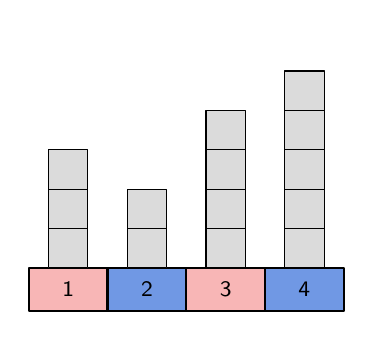
\begin{tikzpicture}[x=1mm,y=1mm,line join=round]
\path (0,0) rectangle (40,36.0);
\draw[thick, fill=slotred] (0,0) rectangle (10,5.5);
\node[font=\footnotesize] at (5.0,2.75) {1};
\draw[fill=black!14] (2.5,5.5) rectangle (7.5,10.5);
\draw[fill=black!14] (2.5,10.5) rectangle (7.5,15.5);
\draw[fill=black!14] (2.5,15.5) rectangle (7.5,20.5);
\draw[thick, fill=slotblue] (10,0) rectangle (20,5.5);
\node[font=\footnotesize] at (15.0,2.75) {2};
\draw[fill=black!14] (12.5,5.5) rectangle (17.5,10.5);
\draw[fill=black!14] (12.5,10.5) rectangle (17.5,15.5);
\draw[thick, fill=slotred] (20,0) rectangle (30,5.5);
\node[font=\footnotesize] at (25.0,2.75) {3};
\draw[fill=black!14] (22.5,5.5) rectangle (27.5,10.5);
\draw[fill=black!14] (22.5,10.5) rectangle (27.5,15.5);
\draw[fill=black!14] (22.5,15.5) rectangle (27.5,20.5);
\draw[fill=black!14] (22.5,20.5) rectangle (27.5,25.5);
\draw[thick, fill=slotblue] (30,0) rectangle (40,5.5);
\node[font=\footnotesize] at (35.0,2.75) {4};
\draw[fill=black!14] (32.5,5.5) rectangle (37.5,10.5);
\draw[fill=black!14] (32.5,10.5) rectangle (37.5,15.5);
\draw[fill=black!14] (32.5,15.5) rectangle (37.5,20.5);
\draw[fill=black!14] (32.5,20.5) rectangle (37.5,25.5);
\draw[fill=black!14] (32.5,25.5) rectangle (37.5,30.5);
\end{tikzpicture}\\[2mm]{\small first \rule{11mm}{0.4pt}\quad second \rule{11mm}{0.4pt}}\end{minipage}}\par\newpage\problem Does the grown-up's plan work on rows of five? Find out who wins each of these colored rows when both players play as well as they can.\par\vspace{4mm}\noindent \begin{minipage}[b]{0.48\linewidth}\centering 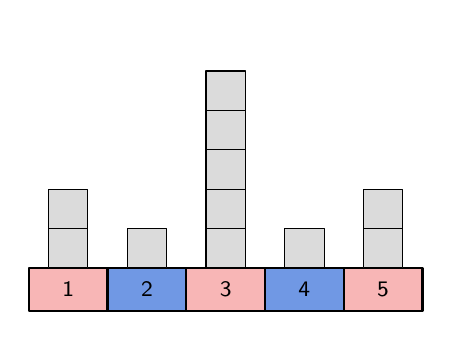
\begin{tikzpicture}[x=1mm,y=1mm,line join=round]
\path (0,0) rectangle (50,36.0);
\draw[thick, fill=slotred] (0,0) rectangle (10,5.5);
\node[font=\footnotesize] at (5.0,2.75) {1};
\draw[fill=black!14] (2.5,5.5) rectangle (7.5,10.5);
\draw[fill=black!14] (2.5,10.5) rectangle (7.5,15.5);
\draw[thick, fill=slotblue] (10,0) rectangle (20,5.5);
\node[font=\footnotesize] at (15.0,2.75) {2};
\draw[fill=black!14] (12.5,5.5) rectangle (17.5,10.5);
\draw[thick, fill=slotred] (20,0) rectangle (30,5.5);
\node[font=\footnotesize] at (25.0,2.75) {3};
\draw[fill=black!14] (22.5,5.5) rectangle (27.5,10.5);
\draw[fill=black!14] (22.5,10.5) rectangle (27.5,15.5);
\draw[fill=black!14] (22.5,15.5) rectangle (27.5,20.5);
\draw[fill=black!14] (22.5,20.5) rectangle (27.5,25.5);
\draw[fill=black!14] (22.5,25.5) rectangle (27.5,30.5);
\draw[thick, fill=slotblue] (30,0) rectangle (40,5.5);
\node[font=\footnotesize] at (35.0,2.75) {4};
\draw[fill=black!14] (32.5,5.5) rectangle (37.5,10.5);
\draw[thick, fill=slotred] (40,0) rectangle (50,5.5);
\node[font=\footnotesize] at (45.0,2.75) {5};
\draw[fill=black!14] (42.5,5.5) rectangle (47.5,10.5);
\draw[fill=black!14] (42.5,10.5) rectangle (47.5,15.5);
\end{tikzpicture}\\[2mm]{\small first \rule{11mm}{0.4pt}\quad second \rule{11mm}{0.4pt}}\end{minipage}\hfill\begin{minipage}[b]{0.48\linewidth}\centering 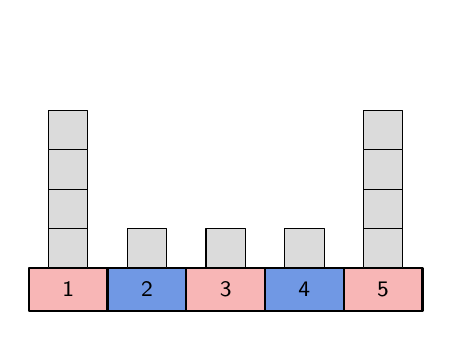
\begin{tikzpicture}[x=1mm,y=1mm,line join=round]
\path (0,0) rectangle (50,36.0);
\draw[thick, fill=slotred] (0,0) rectangle (10,5.5);
\node[font=\footnotesize] at (5.0,2.75) {1};
\draw[fill=black!14] (2.5,5.5) rectangle (7.5,10.5);
\draw[fill=black!14] (2.5,10.5) rectangle (7.5,15.5);
\draw[fill=black!14] (2.5,15.5) rectangle (7.5,20.5);
\draw[fill=black!14] (2.5,20.5) rectangle (7.5,25.5);
\draw[thick, fill=slotblue] (10,0) rectangle (20,5.5);
\node[font=\footnotesize] at (15.0,2.75) {2};
\draw[fill=black!14] (12.5,5.5) rectangle (17.5,10.5);
\draw[thick, fill=slotred] (20,0) rectangle (30,5.5);
\node[font=\footnotesize] at (25.0,2.75) {3};
\draw[fill=black!14] (22.5,5.5) rectangle (27.5,10.5);
\draw[thick, fill=slotblue] (30,0) rectangle (40,5.5);
\node[font=\footnotesize] at (35.0,2.75) {4};
\draw[fill=black!14] (32.5,5.5) rectangle (37.5,10.5);
\draw[thick, fill=slotred] (40,0) rectangle (50,5.5);
\node[font=\footnotesize] at (45.0,2.75) {5};
\draw[fill=black!14] (42.5,5.5) rectangle (47.5,10.5);
\draw[fill=black!14] (42.5,10.5) rectangle (47.5,15.5);
\draw[fill=black!14] (42.5,15.5) rectangle (47.5,20.5);
\draw[fill=black!14] (42.5,20.5) rectangle (47.5,25.5);
\end{tikzpicture}\\[2mm]{\small first \rule{11mm}{0.4pt}\quad second \rule{11mm}{0.4pt}}\end{minipage}\par\vspace{6mm}
\noindent \begin{minipage}[b]{0.48\linewidth}\centering 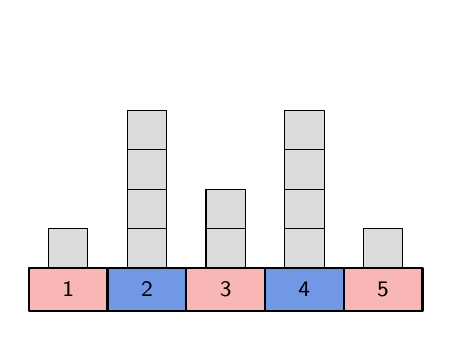
\begin{tikzpicture}[x=1mm,y=1mm,line join=round]
\path (0,0) rectangle (50,36.0);
\draw[thick, fill=slotred] (0,0) rectangle (10,5.5);
\node[font=\footnotesize] at (5.0,2.75) {1};
\draw[fill=black!14] (2.5,5.5) rectangle (7.5,10.5);
\draw[thick, fill=slotblue] (10,0) rectangle (20,5.5);
\node[font=\footnotesize] at (15.0,2.75) {2};
\draw[fill=black!14] (12.5,5.5) rectangle (17.5,10.5);
\draw[fill=black!14] (12.5,10.5) rectangle (17.5,15.5);
\draw[fill=black!14] (12.5,15.5) rectangle (17.5,20.5);
\draw[fill=black!14] (12.5,20.5) rectangle (17.5,25.5);
\draw[thick, fill=slotred] (20,0) rectangle (30,5.5);
\node[font=\footnotesize] at (25.0,2.75) {3};
\draw[fill=black!14] (22.5,5.5) rectangle (27.5,10.5);
\draw[fill=black!14] (22.5,10.5) rectangle (27.5,15.5);
\draw[thick, fill=slotblue] (30,0) rectangle (40,5.5);
\node[font=\footnotesize] at (35.0,2.75) {4};
\draw[fill=black!14] (32.5,5.5) rectangle (37.5,10.5);
\draw[fill=black!14] (32.5,10.5) rectangle (37.5,15.5);
\draw[fill=black!14] (32.5,15.5) rectangle (37.5,20.5);
\draw[fill=black!14] (32.5,20.5) rectangle (37.5,25.5);
\draw[thick, fill=slotred] (40,0) rectangle (50,5.5);
\node[font=\footnotesize] at (45.0,2.75) {5};
\draw[fill=black!14] (42.5,5.5) rectangle (47.5,10.5);
\end{tikzpicture}\\[2mm]{\small first \rule{11mm}{0.4pt}\quad second \rule{11mm}{0.4pt}}\end{minipage}\hfill\begin{minipage}[b]{0.48\linewidth}\centering 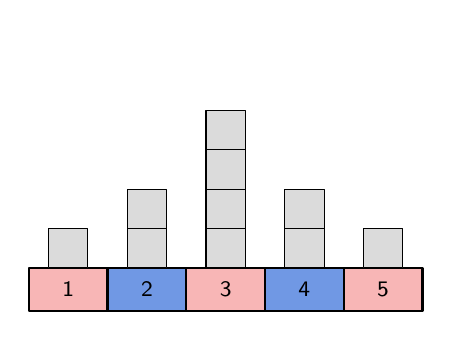
\begin{tikzpicture}[x=1mm,y=1mm,line join=round]
\path (0,0) rectangle (50,36.0);
\draw[thick, fill=slotred] (0,0) rectangle (10,5.5);
\node[font=\footnotesize] at (5.0,2.75) {1};
\draw[fill=black!14] (2.5,5.5) rectangle (7.5,10.5);
\draw[thick, fill=slotblue] (10,0) rectangle (20,5.5);
\node[font=\footnotesize] at (15.0,2.75) {2};
\draw[fill=black!14] (12.5,5.5) rectangle (17.5,10.5);
\draw[fill=black!14] (12.5,10.5) rectangle (17.5,15.5);
\draw[thick, fill=slotred] (20,0) rectangle (30,5.5);
\node[font=\footnotesize] at (25.0,2.75) {3};
\draw[fill=black!14] (22.5,5.5) rectangle (27.5,10.5);
\draw[fill=black!14] (22.5,10.5) rectangle (27.5,15.5);
\draw[fill=black!14] (22.5,15.5) rectangle (27.5,20.5);
\draw[fill=black!14] (22.5,20.5) rectangle (27.5,25.5);
\draw[thick, fill=slotblue] (30,0) rectangle (40,5.5);
\node[font=\footnotesize] at (35.0,2.75) {4};
\draw[fill=black!14] (32.5,5.5) rectangle (37.5,10.5);
\draw[fill=black!14] (32.5,10.5) rectangle (37.5,15.5);
\draw[thick, fill=slotred] (40,0) rectangle (50,5.5);
\node[font=\footnotesize] at (45.0,2.75) {5};
\draw[fill=black!14] (42.5,5.5) rectangle (47.5,10.5);
\end{tikzpicture}\\[2mm]{\small first \rule{11mm}{0.4pt}\quad second \rule{11mm}{0.4pt}}\end{minipage}\par\vspace{6mm}\problem Make up a colored row of six where the red slots and the blue slots hold the same number of cubes, and the first player wins when both players play as well as they can.\par\vspace{6mm}\centerline{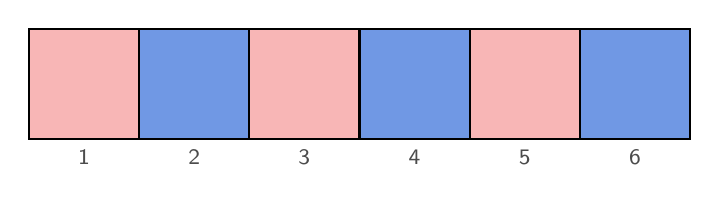
\begin{tikzpicture}[x=1mm,y=1mm]
\draw[thick, fill=slotred] (0,0) rectangle (14,14);
\node[font=\footnotesize, black!70] at (7.0,-2.3) {1};
\draw[thick, fill=slotblue] (14,0) rectangle (28,14);
\node[font=\footnotesize, black!70] at (21.0,-2.3) {2};
\draw[thick, fill=slotred] (28,0) rectangle (42,14);
\node[font=\footnotesize, black!70] at (35.0,-2.3) {3};
\draw[thick, fill=slotblue] (42,0) rectangle (56,14);
\node[font=\footnotesize, black!70] at (49.0,-2.3) {4};
\draw[thick, fill=slotred] (56,0) rectangle (70,14);
\node[font=\footnotesize, black!70] at (63.0,-2.3) {5};
\draw[thick, fill=slotblue] (70,0) rectangle (84,14);
\node[font=\footnotesize, black!70] at (77.0,-2.3) {6};
\end{tikzpicture}}\par\vspace{8mm}\centerline{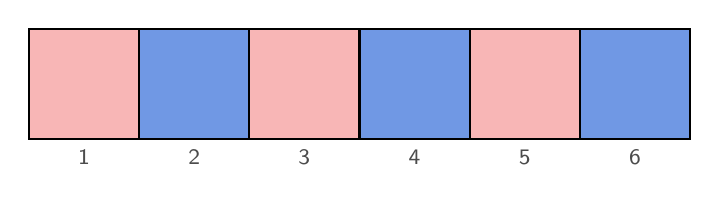
\begin{tikzpicture}[x=1mm,y=1mm]
\draw[thick, fill=slotred] (0,0) rectangle (14,14);
\node[font=\footnotesize, black!70] at (7.0,-2.3) {1};
\draw[thick, fill=slotblue] (14,0) rectangle (28,14);
\node[font=\footnotesize, black!70] at (21.0,-2.3) {2};
\draw[thick, fill=slotred] (28,0) rectangle (42,14);
\node[font=\footnotesize, black!70] at (35.0,-2.3) {3};
\draw[thick, fill=slotblue] (42,0) rectangle (56,14);
\node[font=\footnotesize, black!70] at (49.0,-2.3) {4};
\draw[thick, fill=slotred] (56,0) rectangle (70,14);
\node[font=\footnotesize, black!70] at (63.0,-2.3) {5};
\draw[thick, fill=slotblue] (70,0) rectangle (84,14);
\node[font=\footnotesize, black!70] at (77.0,-2.3) {6};
\end{tikzpicture}}\par\vspace{8mm}\centerline{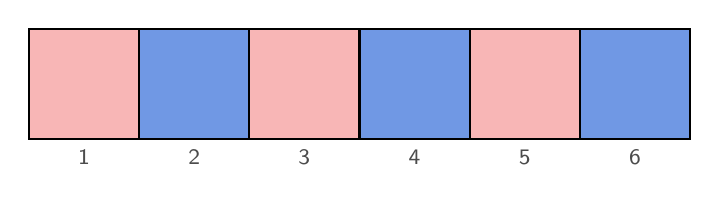
\begin{tikzpicture}[x=1mm,y=1mm]
\draw[thick, fill=slotred] (0,0) rectangle (14,14);
\node[font=\footnotesize, black!70] at (7.0,-2.3) {1};
\draw[thick, fill=slotblue] (14,0) rectangle (28,14);
\node[font=\footnotesize, black!70] at (21.0,-2.3) {2};
\draw[thick, fill=slotred] (28,0) rectangle (42,14);
\node[font=\footnotesize, black!70] at (35.0,-2.3) {3};
\draw[thick, fill=slotblue] (42,0) rectangle (56,14);
\node[font=\footnotesize, black!70] at (49.0,-2.3) {4};
\draw[thick, fill=slotred] (56,0) rectangle (70,14);
\node[font=\footnotesize, black!70] at (63.0,-2.3) {5};
\draw[thick, fill=slotblue] (70,0) rectangle (84,14);
\node[font=\footnotesize, black!70] at (77.0,-2.3) {6};
\end{tikzpicture}}\par\vspace{8mm}
\end{document}
